\documentclass{beamer}

\begin{document}

\begin{frame}
\frametitle{Performance Optimisation}
\begin{itemize}
\item The algorithm must be executed for each pixel.
\item For example: $1920 \times 1080 = 2073600$ pixels.
\item Parallel computing allows simultaneous program execution.
\item Multi-threading allows use of multiple CPU cores. On average CPU has 2-8 cores.
\end{itemize}
\end{frame}


\begin{frame}
\frametitle{The Graphics Processing Unit}
\begin{itemize}
\item Designed primarily for computer graphics.
\item Video games, computer aided design (CAD) machine learning.
\item GPUs have 1,000s - 10,000s of cores.
\item Graphics APIs such as OpenGL, Vulkan, Direct3D, Metal.
\item Rendering pipeline.
\item "Shaders" are programs that execute on the GPU.
\end{itemize}
\end{frame}


\begin{frame}
\frametitle{OpenGL Rendering Pipeline}
\begin{columns}
    \begin{column}{0.5\textwidth}
      \begin{itemize}
        \item Programmer supplies vertices.
        \item Vertex shader program processes them.
        \item Rasterizer breaks down Primatives into Fragments.
        \item Fragment shader colours each pixel individually.
      \end{itemize}
    \end{column}
    \begin{column}{0.5\textwidth}
      \centering
      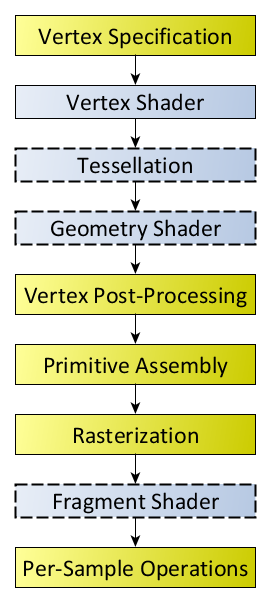
\includegraphics[width=0.6\textwidth]{RenderingPipeline.png}
      \par \tiny {Source: https://www.khronos.org/opengl/wiki\\/Rendering\_Pipeline\_Overview}
    \end{column}
  \end{columns}
\end{frame}

\end{document}
